\documentclass{article}
\usepackage[utf8]{inputenc}
\usepackage{graphicx} % 导入图片
\usepackage{titlesec} % 调整章节标题格式
\usepackage{listings} % 代码格式化
\usepackage{xcolor} % 代码变色
\usepackage{enumitem} % 列表格式化
\usepackage{booktabs} % 三线表
\usepackage{longtable} % 跨页表格
\usepackage{geometry} % 页面布局
\usepackage{ctex} % 支持中文
\usepackage{epstopdf}

\geometry{a4paper, left=2cm, right=2cm, top=2cm, bottom=2cm}
\definecolor{mygreen}{rgb}{0,0.6,0}
\definecolor{mygray}{rgb}{0.5,0.5,0.5}
\definecolor{mymauve}{rgb}{0.58,0,0.82}
\lstset{ %
backgroundcolor=\color{white}, %背景色
basicstyle=\footnotesize\ttfamily, %样式和字体
columns=fullflexible, %字间距
breaklines=true, %代码过长则换行
captionpos=b, % sets the caption-position to bottom
tabsize=4,
commentstyle=\color{mygreen}, %注释颜色
escapeinside={\%*}{(*)}, %特殊自定分隔符
keywordstyle=\color{blue}, %关键字颜色
stringstyle=\color{mymauve}\ttfamily, %字符串颜色
frame=shadowbox, %用方框框住代码块
rulesepcolor=\color{red!20!green!20!blue!20}, %代码块边框颜色
% identifierstyle=\color{red},
numbers=left, %行号在左侧显示
numberstyle=\tiny, %行号字体
% escapeinside=' ', %代码包含中文
xleftmargin=2em,
xrightmargin=2em, 
aboveskip=1em
}

\titleformat{\section}{\normalfont\Large\bfseries}{\S\thesection}{1em}{}
\titleformat{\subsection}{\normalfont\large\bfseries}{\S\thesubsection}{1em}{}

\begin{document}

\begin{center}
   
    
    \huge{智能面容美学量化引擎}\\
    \vspace{1cm}
    

\end{center}

% \pagebreak % 新的一页

\section{引言}
%\includegraphics[width=0.9\textwidth]{image.png}

萝卜白菜,各有所爱。美这个东西,典型的是主观意志的结果。很多东西在我们看来,并不是美的,但是偏偏有人说很美。比如某些人写的那些诗,在很多人看来,臭不可仰,但很多专业人士认为则是写出了专业的美感。真是仁者见仁,智者见智。\par
还有更专业的美感,就像清华美院一样,在国际上看来都是很美的,只是,我和其他很多人,欣赏不了。其实像下图这样美,主要是西方“主流”人认为这是美的,所以他们也认为这是美的。而西方的主流想法,就是他们是主流,我们负责多元,如果我们的美感成为主流,那不是他们变成多元了?所以,美不美,虽然是个主观概念,但由于人群的数量叠加,还有一点主权意识,或思想意识在里面。个人看法,不喜勿喷。\par
那到底怎么才是中国人认为的美?我们是不是可以通过技术手段来验证一下。搜索大量我们认为是美的人脸,比如下图的关之琳、吴倩莲,等等等等,然后建立一个模型,用模型来评判哪些是美的,哪些是不美的。然后再从这些美的人脸里,拼装出一个AI认为是美的人脸,然后再让我们看看,美不美。\par
美不美,应该由人民说了算。\par

\section{问题主体思路分析}
\subsection{数据集搜索}
我们选择了现有的华南理工大学发布的 SCUT-FBP5500-Database数据集
具体信息\par
共5500张分辨率350*350彩色正面人脸,其中2000张亚洲男性,2000张亚洲女性,750张高加索男性,750张高加索女性\par
每张人脸标记有86个特征点,先用ASM模型给出68个特征点,再由志愿者手动调整并添加至86个
调查方法:\par
60名18-27岁(平均21.6岁)的志愿者\par
给随机展示的人脸照片打分(1-5分,越高越好看)\par
展示的照片中有10%会出现两次\par
如果某张照片的两次打分结果相关系数小于0.7,则需要第三次打分\par
最终得分为所有打分的平均分\par
分数分布,大致服从正态分布(黄色线)\par

\subsection{数据预处理}
1.SCUT-FBP5500-Database记录了60个人对每一张照片的评分,意味着每张图片有60个评分。为了得到每张照片的最终得分,我们需要计算这些评分的平均值。\par
2.将所有照片都转成 numpy.ndarray 格式,而 target 则是这张照片的评分。\par
3.对数据集进行切分,切分为训练集和测试集\par

\subsection{模型训练}
1.“加载 Keras 的 ResNet50 预训练模型\par
2.使用均方误差(Mean Squared Error)作为损失函数\par
3.模型将进行 30 轮训练。训练过程中,模型的参数将根据损失函数的梯度进行更新,以最小化损失函数\par

\subsection{模型评测}
1.使用matplotlib库绘制散点图,x轴为“y-train”数据,y轴为模型预测“x-train”数据的输出结果\par
2.按分布情况判断模型好坏决定是否要再增加训练轮数\par
3.并且同时在测试集测试训练效果\par

\subsection{使用模型进行预测}
1.导入需要预测的图片转换为numpy数组,并将图片数据归一化到0-1之间\par
2.预测并打印结果\par





\section{算法分析及输出结果}
\subsection{训练模型所需库文件}
\begin{lstlisting} [language=python]
%matplotlib inline
import os
import matplotlib.pyplot as plt
import matplotlib.image as mpimg
plt.rcParams['font.size'] = 6
plt.rcParams['figure.figsize'] = (6,6)
from collections import Counter
import pandas as pd
import numpy as np
from keras.preprocessing.image import ImageDataGenerator
from keras.models import Sequential
from keras.layers import Dense
from keras.applications import ResNet50
from keras.callbacks import ModelCheckpoint, ReduceLROnPlateau
from keras.models import load_model
from keras.preprocessing.image import array_to_img, img_to_array, load_img
from sklearn.model_selection import train_test_split
\end{lstlisting}
\subsection{数据预处理}
数据来源 :华南理工大学发布的 SCUT-FBP5500-Database 数据集\\
加载数据
\begin{lstlisting} [language=python]
ratings = pd.read_excel('SCUT-FBP5500_with_Landmarks/All_Ratings.xlsx')
ratings.head()
\end{lstlisting}

\begin{tabular}{cccc}% 其中,tabular是表格内容的环境;c表示centering,即文本格式居中;c的个数代表列的个数
\toprule %[2pt]设置线宽
Rater& Filename& Rating& original Rating\\
\midrule %[2pt]
1& CF1.jpg& 3& NaN\\
1& CF10.jpg& 3& NaN\\
1& CF100.jpg& 1& NaN\\
1& CF101.jpg& 2& NaN\\
1& CF102.jpg& 3& NaN\\
\bottomrule %[2pt]     
\end{tabular}

这里记录了60个人对每一张照片的评分,意味着每张图片有60个评分。为了得到每张照片的最终得分,我们需要计算这些评分的平均值。
\begin{lstlisting} [language=python]
# 使用groupby方法按'Filename'列对ratings进行分组,并计算每个组的大小(即每个文件名下的行数)。  
# 然后获取这些组的大小(即每个文件名下的行数)并转换为列表。  
filenames = ratings.groupby('Filename').size().index.tolist()  
# 创建一个空列表,用于存储最终的标签信息。  
labels = []  
# 遍历filenames列表中的每个文件名。  
for filename in filenames:  
    # 根据当前的文件名筛选ratings数据集中的行。  
    df = ratings[ratings['Filename'] == filename]  
    # 使用Counter计算df中'Rating'列的最常出现的评分。most_common(1)返回一个列表,其中包含一个元组,  
    # 该元组的第一个元素是最常出现的评分,第二个元素是该评分的数量。我们只取第一个元素作为最常出现的评分。  
    count = Counter(df['Rating']).most_common(1)[0][0]  
    # 计算df中'Rating'列的平均值,并保留两位小数。  
    score = round(df['Rating'].mean(), 2)  
    # 将当前文件名、最常出现的评分和平均评分作为一个字典添加到labels列表中。  
    labels.append({'Filename': filename, 'most_common': count, 'score': score})  
# 将labels列表转换为DataFrame格式,并命名为labels_df。  
labels_df = pd.DataFrame(labels)  
# 显示labels_df的前几行。  
labels_df.head()
\end{lstlisting}

\begin{tabular}{ccc}% 其中,tabular是表格内容的环境;c表示centering,即文本格式居中;c的个数代表列的个数
\toprule %[2pt]设置线宽
Filename& most\_common& score\\
\midrule %[2pt]
AF1.jpg& 3& 2.33\\
AF10.jpg& 4& 3.43\\
AF100.jpg& 3&2.90\\
AF1000.jpg& 4& 3.97\\
AF1001.jpg& 4&3.73\\
\bottomrule %[2pt]     
\end{tabular}

通过打分来查看评分总体分布
\begin{lstlisting} [language=python]
scores = sorted(labels_df.score.tolist())
\end{lstlisting}
\begin{lstlisting} [language=python]
lv1 = [x for x in scores if x<1]
lv2 = [x for x in scores if x>=1 and x<1.5]
lv3 = [x for x in scores if x>=1.5 and x<2]
lv4 = [x for x in scores if x>=2 and x<2.5]
lv5 = [x for x in scores if x>=2.5 and x<3]
lv6 = [x for x in scores if x>=3 and x<3.5]
lv7 = [x for x in scores if x>=3.5 and x<4]
lv8 = [x for x in scores if x>=4 and x<4.5]
lv9 = [x for x in scores if x>=4.5]
plt.bar(['lv1','lv2','lv3','lv4','lv5','lv6','lv7','lv8','lv9'],
       [len(x) for x in [lv1,lv2,lv3,lv4,lv5,lv6,lv7,lv8,lv9]])
\end{lstlisting}
<BarContainer object of 9 artists>\\

原始数据评分分布图:\\
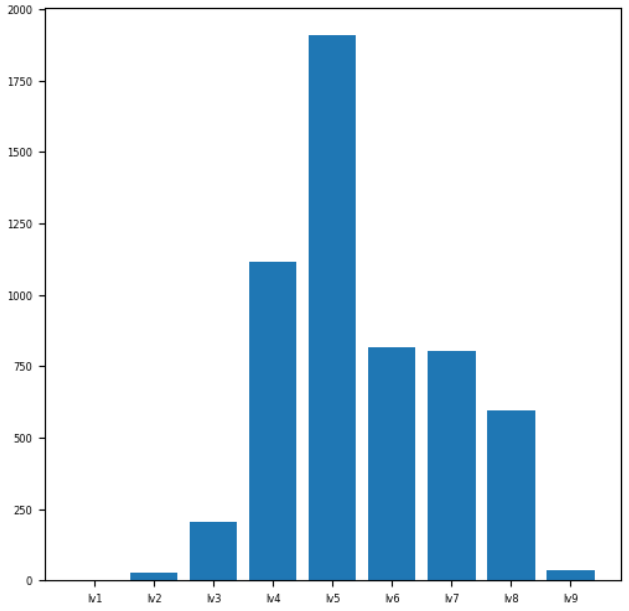
\includegraphics[width=0.98\textwidth]{1.png}

从数据中可以看出,超过半数的评分集中在2~3分的区间,这个范围通常被视为"路人"阶段。相比之下,"盛世美颜"(>4分)和"此颜差矣" (<2分)的评分则相对较少,属于少数派。\par
将所有照片都转成 numpy.ndarray 格式,而 target 则是这张照片的评分。
\subsection{模型切分}
\begin{lstlisting} [language=python]
# 从keras库中导入load_img函数,用于加载图像  
from keras.preprocessing.image import load_img  
# 定义图像的宽度、高度和通道数  
img_width, img_height, channels = 350, 350, 3  
# 定义样本的目录路径  
sample_dir = 'SCUT-FBP5500_with_Landmarks/Images/'  
# 获取目录中的样本数量  
nb_samples = len(os.listdir(sample_dir))  
# 定义输入的形状(宽度、高度和通道数)  
input_shape = (img_width, img_height, channels)  
# 初始化存储所有样本的x和y的数组,这里使用np.empty是为了预先分配空间,提高效率  
x_total = np.empty((nb_samples, img_width, img_height, channels), dtype=np.float32)  
y_total = np.empty((nb_samples, 1), dtype=np.float32)  
# 遍历目录中的每个文件名  
for i, fn in enumerate(os.listdir(sample_dir)):  
    # 使用load_img函数加载图像  
    img = load_img('%s/%s' % (sample_dir, fn))  
    # 将图像转换为数组格式,并重新整形为(高度, 宽度, 通道数)  
    x = img_to_array(img).reshape(img_height, img_width, channels)  
    # 将像素值转换为0-1之间的浮点数,并对255进行归一化处理(这是常见的图像预处理步骤)  
    x = x.astype('float32') / 255.  
    # 从labels_df DataFrame中获取对应的标签值(假设labels_df是根据文件名进行索引的)  
    y = labels_df[labels_df.Filename == fn].score.values  
    # 将标签值转换为浮点数类型  
    y = y.astype('float32')  
    # 将处理后的x和y值存储到x_total和y_total中  
    x_total[i] = x  
    y_total[i] = y
\end{lstlisting}

对数据集进行切分,切分为训练集和测试集
\begin{lstlisting} [language=python]
from sklearn.model_selection import train_test_split
seed = 42
x_train_all, x_test, y_train_all, y_test = train_test_split(x_total, y_total, test_size=0.2, random_state=seed)
x_train, x_val, y_train, y_val = train_test_split(x_train_all, y_train_all, test_size=0.2, random_state=seed)
\end{lstlisting}
\begin{lstlisting} [language=python]
np.save('x_train.npy', x_train)
np.save('y_train.npy', y_train)
np.save('x_val.npy', x_val)
np.save('y_val.npy', y_val)
np.save('x_test.npy', x_test)
np.save('y_test.npy', y_test)
\end{lstlisting}
\begin{lstlisting} [language=python]
# 遍历列表中的每一个元素,其中包含训练数据集、验证集和测试集的特征和标签
for item in [x_train, y_train, x_val, y_val, x_test, y_test]:
    # 打印当前元素的形状  
    print(item.shape)
\end{lstlisting}

(3520, 350, 350, 3)\par
(3520, 1)\par
(880, 350, 350, 3)\par
(880, 1)\par
(1100, 350, 350, 3)\par
(1100, 1)
\subsection{模型建立}
\begin{lstlisting} [language=python]
# 加载训练数据集的特征  
x_train = np.load('x_train.npy')  
# 加载训练数据集的标签  
y_train = np.load('y_train.npy')  
# 加载验证数据集的特征  
x_val = np.load('x_val.npy')  
# 加载验证数据集的标签  
y_val = np.load('y_val.npy')
\end{lstlisting}
\begin{lstlisting} [language=python]
# 遍历列表中的每一个元素,其中包含训练数据集的特征和标签、验证数据集的特征和标签  
for item in [x_train, y_train, x_val, y_val]:  
    # 打印当前元素的形状  
    print(item.shape)
\end{lstlisting}

(3520, 350, 350, 3)\par
(3520, 1)\par
(880, 350, 350, 3)\par
(880, 1)
\begin{lstlisting} [language=python]
# 定义图片的宽度、高度和通道数  
img_width, img_height, channels = 350, 350, 3  
# 定义输入的形状,即模型接受的输入数据的大小  
input_shape = (img_width, img_height, channels)
\end{lstlisting}

以下是对“加载 Keras 的 ResNet50 预训练模型,去掉最后的 softmax 层,然后再加上一层 dense 全连接层,将 ResNet50 模型的其余参数设为不可训练,也就是先直接训练最后的 dense 层的参数;因为是做回归,所以损失函数我们使用 mse”这段话的润色:\par
我们首先加载 Keras 的 ResNet50 预训练模型,然后去掉其最后的 softmax 层。接着,我们添加一层 dense 全连接层以构建我们的模型。为了确保模型的性能,我们将 ResNet50 模型的其余参数设为不可训练,仅专注于训练新增的 dense 层的参数。由于我们正在进行回归任务,因此选择均方误差(mse)作为损失函数。\par
from keras.applications import ResNet50:从 Keras 的 applications 模块中导入 ResNet50 模型。Keras 是一个流行的深度学习框架,ResNet50 是一个预训练的深度残差网络模型。 resnet = ResNet50(include\_top = False, pooling = 'avg', input\_shape = input\_shape):创建一个 ResNet50 模型实例,不包括顶部的全连接层(include\_top = False),使用平均池化(pooling = 'avg'),并设置输入形状为之前定义的 input\_shape。 model = Sequential():创建一个 Sequential 模型实例,这是一个线性堆叠模型的容器。 model.add(resnet):将预训练的 ResNet50 模型添加到 Sequential 模型中。 model.add(Dense(1)):在 ResNet50 模型后面添加一个全连接层(或称为密集层),输出单元数为 1。这里,我们将 ResNet50 的输出作为输入,并添加一个全连接层来执行回归任务。 model.layers[0].trainable = False:将 Sequential 模型中的第一层设置为不可训练(固定参数)。在这里,第一层是 ResNet50 模型。通过设置 trainable = False,我们告诉 Keras 在训练过程中不更新这个层的参数。这样做的目的是为了保留 ResNet50 模型的预训练权重,同时只训练新添加的全连接层。 model.summary():打印模型的摘要,包括每一层的输出形状、参数数量等。这对于理解和调试模型非常有用。
\begin{lstlisting} [language=python]
# 从Keras库中导入ResNet50模型  
from keras.applications import ResNet50  
# 创建一个ResNet50模型实例,不包括顶部的全连接层(只使用卷积层和池化层),使用平均池化,输入形状为之前定义的input_shape  
resnet = ResNet50(include_top=False, pooling='avg', input_shape=input_shape)   
# 创建一个Sequential模型实例  
model = Sequential()    
# 将ResNet50模型添加到Sequential模型中  
model.add(resnet)    
# 在ResNet50模型后面添加一个全连接层,输出单元数为1(即回归问题的一个输出)  
model.add(Dense(1))   
# 将Sequential模型中的第一层设置为不可训练(固定参数)  
model.layers[0].trainable = False    
# 打印模型的摘要,包括每一层的输出形状、参数数量等  
model.summary()
\end{lstlisting}



Model: "sequential"\par

\begin{tabular}{ccc}% 其中,tabular是表格内容的环境;c表示centering,即文本格式居中;c的个数代表列的个数
\toprule %[2pt]设置线宽
Layer (type)& Output Shape& Param \#\\
\midrule %[2pt]
resnet50 (Functional)& (None, 2048)& 23587712\\
\\
dense (Dense)& (None, 1)& 2049\\
\\
\bottomrule %[2pt]     
\end{tabular}\par
\begin{tabular}{l}
\toprule %[2pt]设置线宽
Total params: 23589761 (89.99 MB)\\
Trainable params: 2049 (8.00 KB)\\
Non-trainable params: 23587712 (89.98 MB)\\
\bottomrule %[2pt]  
\end{tabular}

\subsection{模型训练}
\begin{lstlisting} [language=python]
# 使用均方误差作为损失函数,Adam优化器进行优化  
model.compile(loss='mse', optimizer='adam')  
  
# 使用32个样本作为一个批次进行训练,x_train是输入数据,y_train是标签数据,训练30轮  
history = model.fit(batch_size=32, x=x_train, y=y_train, epochs=30)
\end{lstlisting}

model.compile(loss = 'mse', optimizer = 'adam'):这一行代码用于配置模型的训练过程。loss = 'mse' 表示使用均方误差(Mean Squared Error)作为损失函数,这是回归问题的常用损失函数。optimizer = 'adam' 表示使用 Adam 优化器,这是一个流行的梯度下降优化算法,通常在深度学习模型中表现良好。 model.fit(batch\_size = 32, x = x\_train, y = y\_train, epochs = 30):这一行代码用于训练模型。batch\_size = 32 表示每个批次使用 32 个样本进行训练。x = x\_train 和 y = y\_train 分别表示训练数据的输入和标签。epochs = 30 表示模型将进行 30 轮训练。训练过程中,模型的参数将根据损失函数的梯度进行更新,以最小化损失函数。训练结束后,返回的 history 对象将包含训练过程中的各种历史记录和指标。\par

Epoch 1/30\par
110/110 [==============================] - 183s 2s/step - loss: 0.5195\par
Epoch 2/30\par
110/110 [==============================] - 177s 2s/step - loss: 0.4675\par
Epoch 3/30\par
110/110 [==============================] - 177s 2s/step - loss: 0.4377\par
Epoch 4/30\par
110/110 [==============================] - 177s 2s/step - loss: 0.4343\par
Epoch 5/30\par
110/110 [==============================] - 177s 2s/step - loss: 0.4238\par
Epoch 6/30\par
110/110 [==============================] - 177s 2s/step - loss: 0.4064\par
Epoch 7/30\par
110/110 [==============================] - 177s 2s/step - loss: 0.4025\par
Epoch 8/30\par
110/110 [==============================] - 177s 2s/step - loss: 0.4016\par
Epoch 9/30\par
110/110 [==============================] - 177s 2s/step - loss: 0.3957\par
Epoch 10/30\par
110/110 [==============================] - 177s 2s/step - loss: 0.3919\par
Epoch 11/3\par
110/110 [==============================] - 177s 2s/step - loss: 0.3839\par
Epoch 12/30\par
110/110 [==============================] - 177s 2s/step - loss: 0.3853\par
Epoch 13/30\par
110/110 [==============================] - 177s 2s/step - loss: 0.4096\par
Epoch 14/30\par
110/110 [==============================] - 177s 2s/step - loss: 0.3851\par
Epoch 15/30\par
110/110 [==============================] - 177s 2s/step - loss: 0.3748\par
Epoch 16/30\par
110/110 [==============================] - 177s 2s/step - loss: 0.3732\par
Epoch 17/30\par
110/110 [==============================] - 177s 2s/step - loss: 0.3796\par
Epoch 18/30\par
110/110 [==============================] - 177s 2s/step - loss: 0.3827\par
Epoch 19/30\par
110/110 [==============================] - 177s 2s/step - loss: 0.3735\par
Epoch 20/30\par
110/110 [==============================] - 177s 2s/step - loss: 0.3621\par
Epoch 21/30\par
110/110 [==============================] - 177s 2s/step - loss: 0.3663\par
Epoch 22/30\par
110/110 [==============================] - 177s 2s/step - loss: 0.3664\par
Epoch 23/30\par
110/110 [==============================] - 177s 2s/step - loss: 0.3722\par
Epoch 24/30\par
110/110 [==============================] - 177s 2s/step - loss: 0.3650\par
Epoch 25/30\par
110/110 [==============================] - 177s 2s/step - loss: 0.3671\par
Epoch 26/30\par
110/110 [==============================] - 177s 2s/step - loss: 0.3579\par
Epoch 27/30\par
110/110 [==============================] - 177s 2s/step - loss: 0.3544\par
Epoch 28/30\par
110/110 [==============================] - 177s 2s/step - loss: 0.3831\par
Epoch 29/30\par
110/110 [==============================] - 177s 2s/step - loss: 0.3640\par
Epoch 30/30\par
110/110 [==============================] - 177s 2s/step - loss: 0.3584\par
\begin{lstlisting} [language=python]
# 设置matplotlib的图形大小为6x6英寸  
plt.rcParams['figure.figsize'] = (6,6)  
# 从训练历史中提取训练损失  
loss = history.history['loss']  
# 创建一个从1到loss长度(包含)的整数序列,表示训练的轮数  
epochs = range(1, len(loss) + 1)   
# 创建一个新的图形  
plt.figure()  
# 设置图形的标题为“Training loss”  
plt.title('Training loss')  
# 在图形上绘制训练损失随轮数的变化曲线,线颜色为红色,并添加图例  
plt.plot(epochs, loss, 'red', label='Training loss')  
# 显示图例  
plt.legend()  
# 显示图形  
plt.show()
\end{lstlisting}
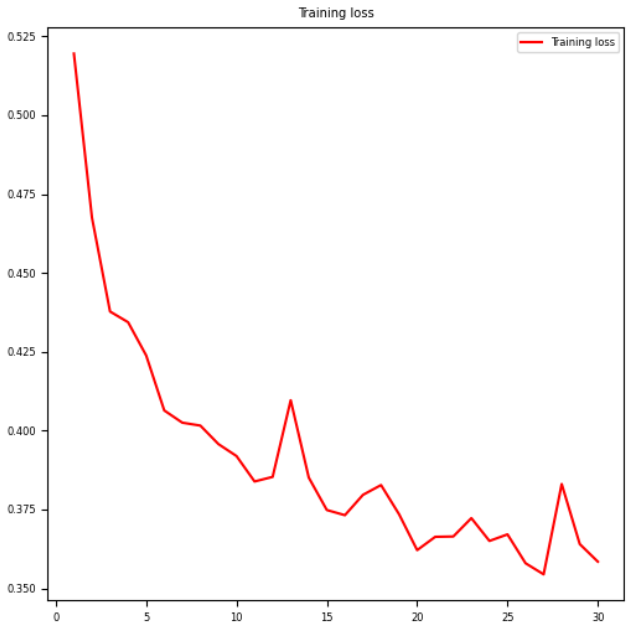
\includegraphics[width=0.98\textwidth]{2.png}

30 个 epochs 之后,loss 下降到 0.3 左右:
\begin{lstlisting} [language=python]
# 使用matplotlib库绘制散点图,x轴为y_train数据,y轴为模型预测x_train数据的输出结果  
plt.scatter(y_train, model.predict(x_train))
\end{lstlisting}
110/110 [==============================] - 178s 2s/step\\
<matplotlib.collections.PathCollection at 0x1b19985b4d0>\\
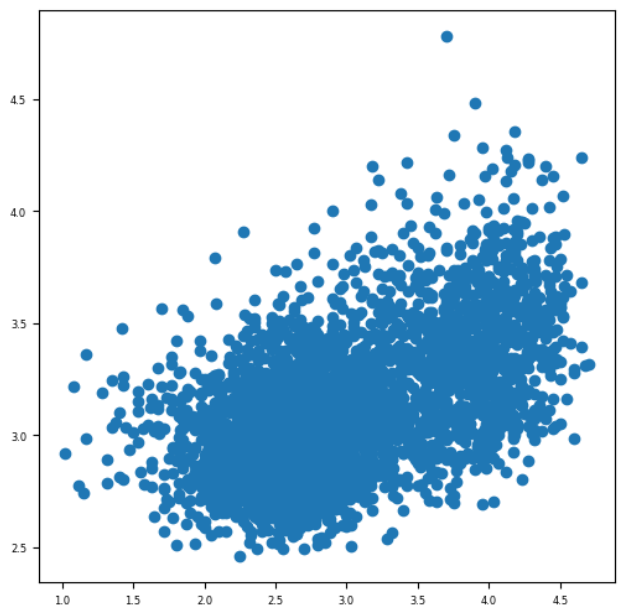
\includegraphics[width=0.98\textwidth]{3.png}

数据分布混乱\par
查阅文献,将 ResNet50 的参数设置为可训练,然后再训练 30 个 epochs,设置了 checkpoint callback,将验证集的 loss 设为监控项,保存该值最低的模型:
\begin{lstlisting} [language=python]
# 定义模型检查点的文件路径格式  
filepath="{epoch:02d}-{val_loss:.2f}.h5"  
# 定义模型检查点回调,用于在训练过程中保存模型  
checkpoint = ModelCheckpoint(filepath, monitor='val_loss', verbose=1, save_best_only=True, mode='min')  
# 定义学习率调整回调,用于当验证损失不再下降时降低学习率  
reduce_learning_rate = ReduceLROnPlateau(monitor='loss',  
                                         factor=0.1,  # 学习率降低的倍数  
                                         patience=2,  # 连续多少个周期(epoch)后,学习率才降低  
                                         cooldown=2,  # 学习率降低后,保持多少个周期(epoch)不变  
                                         min_lr=0.00001,  # 允许的最小学习率  
                                         verbose=1)  
  
# 定义回调列表,包含模型检查点和学率调整回调  
callback_list = [checkpoint, reduce_learning_rate]
\end{lstlisting}

filepath = "{epoch:02d}-{val\_loss:.2f}.h5":定义了模型检查点文件的命名格式。其中,{epoch:02d} 表示格式化当前训练的轮数(epoch)为两位数,{val\_loss:.2f} 表示格式化验证损失值为两位小数。这样,文件名将类似于 03-0.34.h5。 ModelCheckpoint:是一个回调函数,用于在训练过程中保存模型。filepath 参数定义了保存的文件名或路径,monitor = 'val\_loss' 参数指定了要监视的指标(这里是验证损失),verbose = 1 参数表示在控制台输出日志信息,save\_best\_only = True 表示只保存验证损失最小(或最大)的那个模型,mode = 'min' 表示我们要最小化验证损失。 ReduceLROnPlateau:也是一个回调函数,用于当验证损失不再下降时降低学习率。参数 factor = 0.1 表示学习率降低的倍数,patience = 2 表示连续多少个周期(epoch)后,学习率才降低,cooldown = 2 表示学习率降低后,保持多少个周期(epoch)不变,min\_lr = 0.00001 表示允许的最小学习率,verbose = 1 表示在控制台输出日志信息。
\begin{lstlisting} [language=python]
# 将模型的第一层设置为可训练,这意味着在训练过程中,这一层的权重将会更新。  
model.layers[0].trainable = True  
# 使用均方误差损失函数(MSE)和Adam优化器来编译模型。这表示模型将使用这些设置进行训练。  
model.compile(loss='mse', optimizer='adam')  
# 使用训练数据x_train和y_train来拟合模型,并将每个数据分批为大小为8的批次进行训练。  
# 训练将进行10个周期(epochs)。  
# 同时,使用验证数据x_val和y_val来评估模型在每个周期的表现。  
# 回调函数(callback_list)将在训练过程中执行一些额外的操作,例如保存模型的最佳权重等。  
history = model.fit(x=x_train,   
                    y=y_train,   
                    batch_size=8,  
                    epochs=10,  
                    validation_data=(x_val, y_val),  
                    callbacks=callback_list)
\end{lstlisting}
Epoch 1/10\\
440/440 [==============================] - ETA: 0s - loss: 3.5156\\
Epoch 1: val\_loss improved from inf to 7.82225, saving model to 01-7.82.h5\\
440/440 [==============================] - 595s 1s/step - loss: 3.5156 - val\_loss: 7.8222 - lr: 0.0010\\
Epoch 2/10\\
440/440 [==============================] - ETA: 0s - loss: 0.3305\\
Epoch 2: val\_loss improved from 7.82225 to 1.20452, saving model to 02-1.20.h5\\
440/440 [==============================] - 569s 1s/step - loss: 0.3305 - val\_loss: 1.2045 - lr: 0.0010\\
Epoch 3/10\\
440/440 [==============================] - ETA: 0s - loss: 0.2552\\
Epoch 3: val\_loss did not improve from 1.20452\\
440/440 [==============================] - 570s 1s/step - loss: 0.2552 - val\_loss: 2.1555 - lr: 0.0010\\
Epoch 4/10\\
440/440 [==============================] - ETA: 0s - loss: 0.2074\\
Epoch 4: val\_loss improved from 1.20452 to 0.21785, saving model to 04-0.22.h5\\
440/440 [==============================] - 570s 1s/step - loss: 0.2074 - val\_loss: 0.2178 - lr: 0.0010\\
Epoch 5/10\\
440/440 [==============================] - ETA: 0s - loss: 0.1893\\
Epoch 5: val\_loss improved from 0.21785 to 0.18952, saving model to 05-0.19.h5\\
440/440 [==============================] - 570s 1s/step - loss: 0.1893 - val\_loss: 0.1895 - lr: 0.0010\\
Epoch 6/10\\
440/440 [==============================] - ETA: 0s - loss: 0.1751\\
Epoch 6: val\_loss did not improve from 0.18952\\
440/440 [==============================] - 569s 1s/step - loss: 0.1751 - val\_loss: 0.5590 - lr: 0.0010\\
Epoch 7/10\\
440/440 [==============================] - ETA: 0s - loss: 0.1584\\
Epoch 7: val\_loss did not improve from 0.18952\\
440/440 [==============================] - 569s 1s/step - loss: 0.1584 - val\_loss: 0.2483 - lr: 0.0010\\
Epoch 8/10\\
440/440 [==============================] - ETA: 0s - loss: 0.1742\\
Epoch 8: val\_loss did not improve from 0.18952\\
440/440 [==============================] - 569s 1s/step - loss: 0.1742 - val\_loss: 1.0064 - lr: 0.0010\\
Epoch 9/10\\
440/440 [==============================] - ETA: 0s - loss: 0.1351\\
Epoch 9: val\_loss did not improve from 0.18952\\
440/440 [==============================] - 570s 1s/step - loss: 0.1351 - val\_loss: 0.3617 - lr: 0.0010\\
Epoch 10/10\\
440/440 [==============================] - ETA: 0s - loss: 0.1255\\
Epoch 10: val\_loss did not improve from 0.18952\\
440/440 [==============================] - 570s 1s/step - loss: 0.1255 - val\_loss: 0.2349 - lr: 0.0010\\

\begin{lstlisting} [language=python]
from keras.models import load_model
# 最优模型加载
best_model = load_model('05-0.19.h5')
\end{lstlisting}
\begin{lstlisting} [language=python]
# 使用matplotlib的scatter函数来绘制散点图,x轴是训练数据集y_train的标签值,y轴是最佳模型对训练数据集x_train的预测值。  
plt.scatter(y_train, best_model.predict(x_train))  
# 使用plot函数在同一张图上绘制红色的点('ro'表示红色圆点),x轴和y轴的值都是训练数据集y_train的标签值,表示原始数据点。  
plt.plot(y_train, y_train, 'ro')
\end{lstlisting}
110/110 [==============================] - 180s 2s/step\\
[<matplotlib.lines.Line2D at 0x1b6ddd40590>]\\
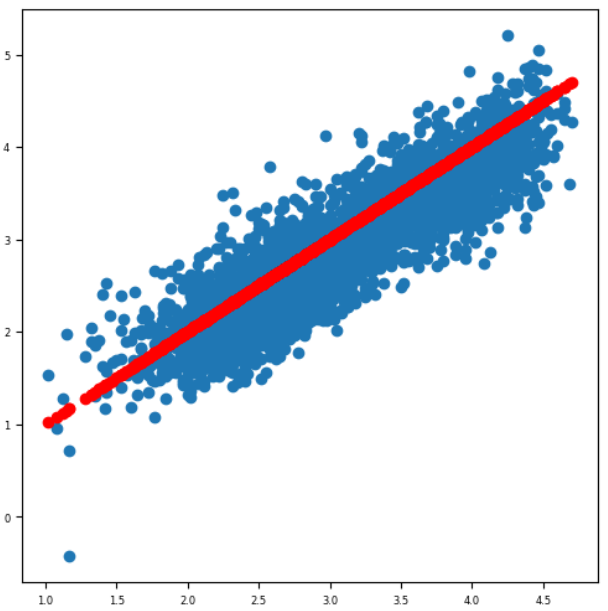
\includegraphics[width=0.98\textwidth]{4.png}\\
\begin{lstlisting} [language=python]
# 使用matplotlib的scatter函数来绘制散点图,x轴是验证数据集y_val的标签值,y轴是最佳模型对验证数据集x_val的预测值。  
plt.scatter(y_val, best_model.predict(x_val))  
# 使用plot函数在同一张图上绘制红色的点('ro'表示红色圆点),x轴和y轴的值都是验证数据集y_val的标签值,表示原始数据点。  
plt.plot(y_val, y_val, 'ro')
\end{lstlisting}
28/28 [==============================] - 46s 2s/step\\
[<matplotlib.lines.Line2D at 0x1b9a80ec890>]\\
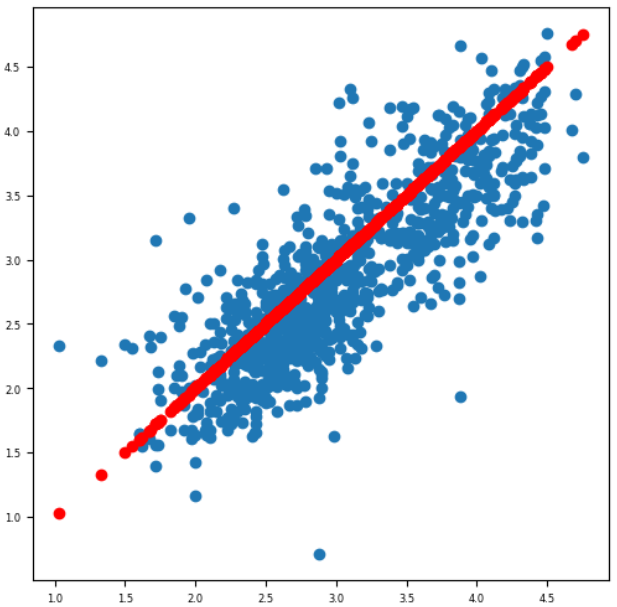
\includegraphics[width=0.98\textwidth]{5.png}

在测试集上效果不错
\begin{lstlisting} [language=python]
x_test = np.load('x_test.npy')
y_test = np.load('y_test.npy')
\end{lstlisting}
\begin{lstlisting} [language=python]
# 使用最佳模型(best_model)在测试数据集(x_test, y_test)上进行评估。  
# 这会返回模型在测试数据集上的损失值和任何可用的评价指标。  
best_model.evaluate(x=x_test, y=y_test)
\end{lstlisting}
35/35 [==============================] - 57s 2s/step - loss: 0.1992\\
0.19919565320014954\\
\begin{lstlisting} [language=python]
# 使用matplotlib的scatter函数绘制散点图,x轴是测试数据集y_test的真实标签值,y轴是最佳模型对测试数据集x_test的预测值。  
plt.scatter(y_test, best_model.predict(x_test))  
# 使用plot函数在同一张图上绘制红色的点('ro'表示红色圆点),x轴和y轴的值都是测试数据集y_test的真实标签值,表示原始数据点。  
plt.plot(y_test, y_test, 'ro')
\end{lstlisting}
35/35 [==============================] - 56s 2s/step\\
[<matplotlib.lines.Line2D at 0x1b6dff97fd0>]\\
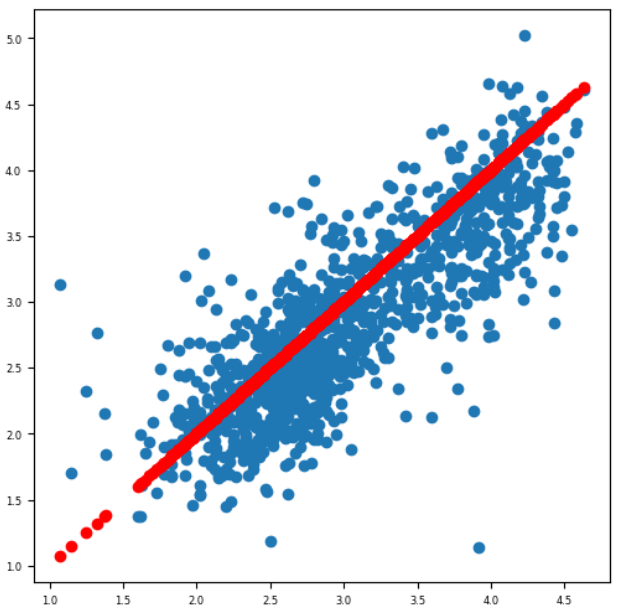
\includegraphics[width=0.98\textwidth]{6.png}\\
\begin{lstlisting} [language=python]
# 使用最佳模型(best_model)对测试数据集(x_test)进行预测,并将预测结果存储在scores变量中。  
scores = best_model.predict(x_test)  
# 将scores从NumPy数组转换为Python列表,然后使用列表推导式提取每个预测结果的第一个元素。    
# [x[0] for x in scores.tolist()]将返回一个形状为(n,)的一维Python列表,其中每个元素都是scores中相应元素的第一个元素。  
scores = [x[0] for x in scores.tolist()]
\end{lstlisting}
35/35 [==============================] - 56s 2s/step
\begin{lstlisting} [language=python]
lv1 = [x for x in scores if x<1]
lv2 = [x for x in scores if x>=1 and x<1.5]
lv3 = [x for x in scores if x>=1.5 and x<2]
lv4 = [x for x in scores if x>=2 and x<2.5]
lv5 = [x for x in scores if x>=2.5 and x<3]
lv6 = [x for x in scores if x>=3 and x<3.5]
lv7 = [x for x in scores if x>=3.5 and x<4]
lv8 = [x for x in scores if x>=4 and x<4.5]
lv9 = [x for x in scores if x>=4.5]
plt.bar(['lv1','lv2','lv3','lv4','lv5','lv6','lv7','lv8','lv9'],
       [len(x) for x in [lv1,lv2,lv3,lv4,lv5,lv6,lv7,lv8,lv9]])
\end{lstlisting}
<BarContainer object of 9 artists>\\
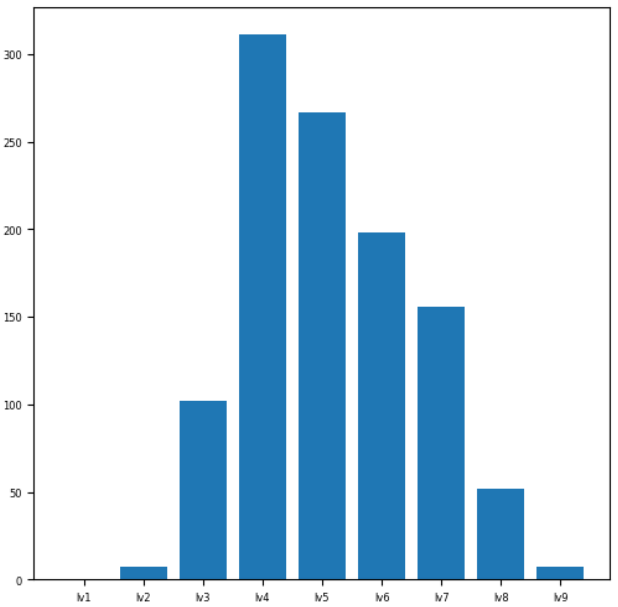
\includegraphics[width=0.98\textwidth]{7.png}\\
查看测试集分布,依旧满足正态分布



\subsection{部分数据结果对比展示}
\begin{lstlisting} [language=python]
# 设置matplotlib的全局参数  
# 'font.size': 字体大小  
# 'figure.figsize': 图形大小  
plt.rcParams['font.size'] = 9  
plt.rcParams['figure.figsize'] = (9,9)  
  
# 导入random模块中的randint函数,用于生成随机整数  
from random import randint  
  
# 获取测试数据集的数量  
nb_test_samples = x_test.shape[0]  
# 定义图形的行数和列数  
nb_rows, nb_cols = 5, 5  
  
# 定义一个函数来检查测试结果并可视化部分样本  
def check_test_result():  
    # 循环遍历每一张子图(即每一个样本)  
    for k in range(nb_rows * nb_cols):  
        # 随机选择一个测试样本的索引  
        i = randint(0, nb_test_samples - 1)  
        # 使用模型预测该样本的标签(注意:这里假设最佳模型的输出是分类概率)  
        predicted = best_model.predict(x_test[i].reshape((1,) + x_test[i].shape))  
        # 设置当前子图的位置  
        plt.subplot(nb_rows, nb_cols, k+1)  
        # 显示样本图像  
        plt.imshow(x_test[i])  
        # 设置图像标题,显示预测概率和真实标签  
        plt.title("p:%.2f a:%.2f" % (predicted[0][0], y_test[i]))  
        # 不显示坐标轴  
        plt.axis('off')  
# 调用函数来检查并可视化测试结果  
check_test_result()
\end{lstlisting}
1/1 [==============================] - 0s 152ms/step\\
1/1 [==============================] - 0s 117ms/step\\
1/1 [==============================] - 0s 121ms/step\\
1/1 [==============================] - 0s 118ms/step\\
1/1 [==============================] - 0s 116ms/step\\
1/1 [==============================] - 0s 121ms/step\\
1/1 [==============================] - 0s 121ms/step\\
1/1 [==============================] - 0s 119ms/step\\
1/1 [==============================] - 0s 121ms/step\\
1/1 [==============================] - 0s 122ms/step\\
1/1 [==============================] - 0s 118ms/step\\
1/1 [==============================] - 0s 122ms/step\\
1/1 [==============================] - 0s 118ms/step\\
1/1 [==============================] - 0s 121ms/step\\
1/1 [==============================] - 0s 119ms/step\\
1/1 [==============================] - 0s 118ms/step\\
1/1 [==============================] - 0s 125ms/step\\
1/1 [==============================] - 0s 119ms/step\\
1/1 [==============================] - 0s 129ms/step\\
1/1 [==============================] - 0s 119ms/step\\
1/1 [==============================] - 0s 129ms/step\\
1/1 [==============================] - 0s 128ms/step\\
1/1 [==============================] - 0s 121ms/step\\
1/1 [==============================] - 0s 119ms/step\\
1/1 [==============================] - 0s 122ms/step\\

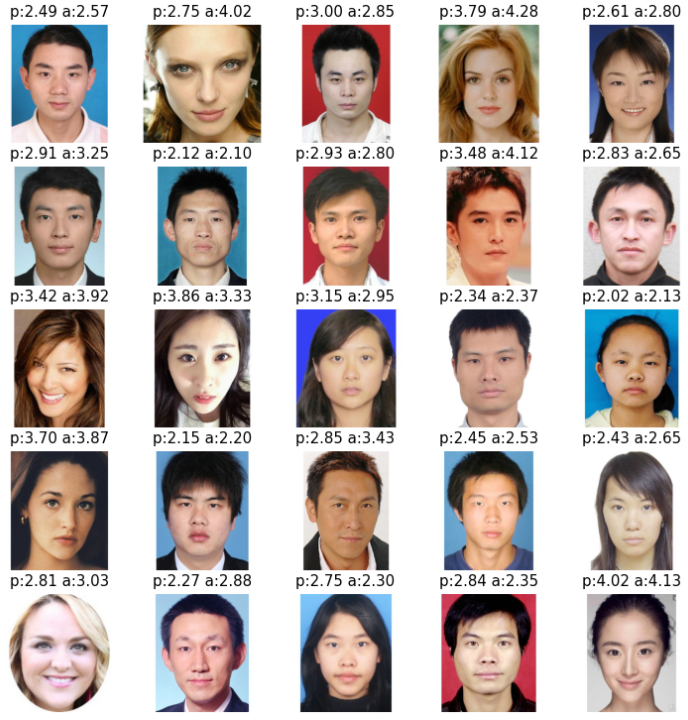
\includegraphics[width=0.98\textwidth]{8.png}

部分测试结果与对应结果相差不大
\subsection{预测函数的实现}
\begin{lstlisting} [language=python]
# 设置matplotlib的字体大小为6  
plt.rcParams['font.size'] = 6  
# 设置图形的尺寸为6x6单位  
plt.rcParams['figure.figsize'] = (6,6)  
# 加载图片'ishihara.jpg',这通常用于检测颜色盲  
img = load_img('ishihara.jpg')  
# 使用matplotlib显示图片  
plt.imshow(img)  
# 将图片数据转换为numpy数组,并重新整形为img_height x img_width x channels的形状   
test_x = np.array(img).reshape(img_height, img_width, channels)  
# 将图片数据归一化到0-1之间  
test_x = test_x / 255.  
# 再次改变数组的形状,以满足模型的输入要求  
test_x = test_x.reshape((1,) + test_x.shape)  
# 使用best_model来预测图片的颜色盲类型  
predicted = best_model.predict(test_x)  
# 打印预测结果  
print("predicted: %.2f" % predicted[0][0])
\end{lstlisting}
1/1 [==============================] - 0s 136ms/step\\
predicted: 3.45\\
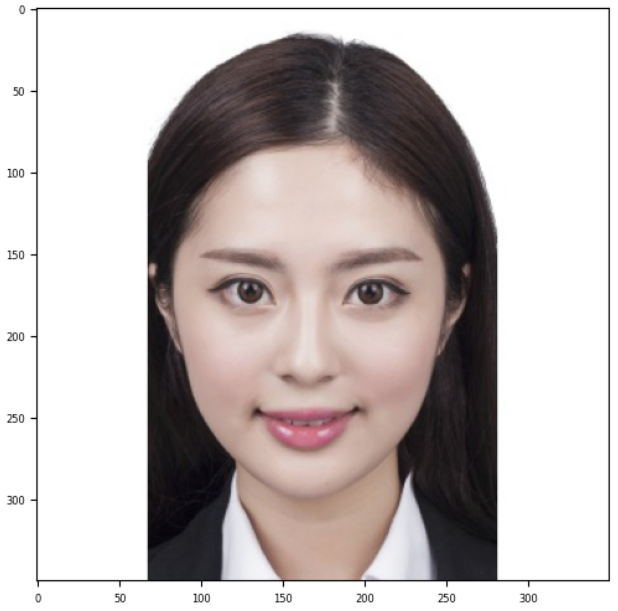
\includegraphics[width=0.98\textwidth]{9.png}


\subsection{可视化窗口的实现}
\subsubsection{可视化窗口QT配置}

\begin{lstlisting} [language=python]
from PyQt5 import QtCore, QtGui, QtWidgets
class Ui_Form(object):
    def setupUi(self, Form):
        Form.setObjectName("人脸打分")
        Form.resize(751, 756)
        self.widget = QtWidgets.QWidget(Form)
        self.widget.setGeometry(QtCore.QRect(40, 90, 681, 581))
        self.widget.setObjectName("widget")
        self.verticalLayout = QtWidgets.QVBoxLayout(self.widget)
        self.verticalLayout.setContentsMargins(0, 0, 0, 0)
        self.verticalLayout.setObjectName("verticalLayout")
        self.picture = QtWidgets.QLabel(self.widget)
        self.picture.setObjectName("picture")
        self.verticalLayout.addWidget(self.picture)
        self.choosepicture = QtWidgets.QPushButton(self.widget)
        self.choosepicture.setObjectName("choosepicture")
        self.verticalLayout.addWidget(self.choosepicture)
        self.decide = QtWidgets.QPushButton(self.widget)
        self.decide.setObjectName("decide")
        self.verticalLayout.addWidget(self.decide)
        self.dafen = QtWidgets.QLabel(self.widget)
        self.dafen.setObjectName("dafen")
        self.verticalLayout.addWidget(self.dafen)
        self.verticalLayout.setStretch(0, 1)
        self.verticalLayout.setStretch(1, 1)
        self.verticalLayout.setStretch(2, 1)

        self.retranslateUi(Form)
        QtCore.QMetaObject.connectSlotsByName(Form)

    def retranslateUi(self, Form):
        _translate = QtCore.QCoreApplication.translate
        Form.setWindowTitle(_translate("Form", "Form"))
        self.picture.setText(_translate("Form", "图片"))
        self.choosepicture.setText(_translate("Form", "选择图片"))
        self.decide.setText(_translate("Form", "确定"))
        self.dafen.setText(_translate("Form", "打分"))
\end{lstlisting}
\subsubsection{可视化加载}
\begin{lstlisting}[language=python]
import cv2
import numpy as np
from PyQt5.QtWidgets import QApplication, QWidget, QMessageBox, QFileDialog, QLabel,QMainWindow
from PyQt5.QtGui import QPixmap
from PyQt5.QtCore import Qt
from untitled import Ui_Form
import sys
from keras.models import load_model
import numpy as np
import matplotlib.pyplot as plt
from keras.preprocessing.image import load_img
class MainWindow(QMainWindow):
    def __init__(self):
        super().__init__()
        self.ui = Ui_Form()
        self.ui.setupUi(self)
        self.file_path=""
        self.ui.choosepicture.clicked.connect(self.choosepicture)
        self.ui.decide.clicked.connect(self.dafen)
    def choosepicture(self):
        self.file_path, _ = QFileDialog.getOpenFileName(self, "选择图片", "", "Images (*.png *.jpg)")
        if self.file_path:
            MainWindow.global_image_path = self.file_path
            pixmap = QPixmap(self.file_path)
            self.ui.picture.setPixmap(pixmap.scaled(self.ui.picture.size()))
    def dafen(self):
        img_width, img_height, channels = 350, 350, 3
        best_model = load_model('./05-0.19.h5')
        # 设置matplotlib的字体大小为6
        plt.rcParams['font.size'] = 6
        # 设置图形的尺寸为6x6单位
        plt.rcParams['figure.figsize'] = (6, 6)
        # 加载图片'ishihara.jpg',这通常用于检测颜色盲
        img = load_img(MainWindow.global_image_path)
        # 使用matplotlib显示图片
        plt.imshow(img)
        # 将图片数据转换为numpy数组,并重新整形为img_height x img_width x channels的形状
        test_x = np.array(img).reshape(img_height, img_width, channels)
        # 将图片数据归一化到0-1之间
        test_x = test_x / 255.
        # 再次改变数组的形状,以满足模型的输入要求
        test_x = test_x.reshape((1,) + test_x.shape)
        # 使用best_model来预测图片的颜色盲类型
        predicted = best_model.predict(test_x)
        # 打印预测结果
        self.ui.dafen.setText("predicted: %.2f" % predicted[0][0])
if __name__ == '__main__':
    app = QApplication(sys.argv)
    window = MainWindow()
    window.show()
    sys.exit(app.exec_())
\end{lstlisting}
\subsubsection{可视化界面展示}
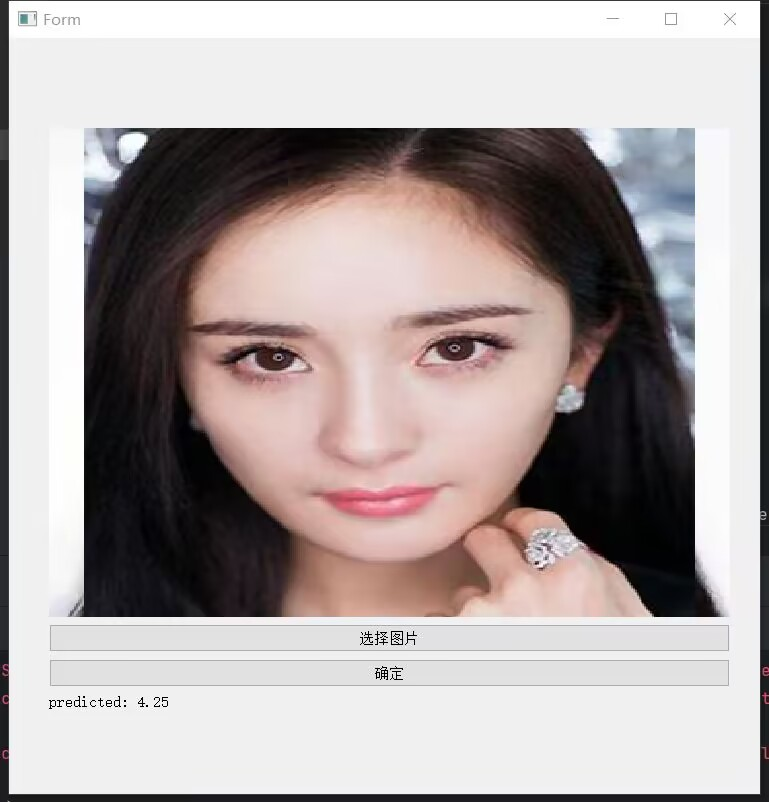
\includegraphics[width=0.98\textwidth]{0.png}





\bibliographystyle{ieeetr}
{\small}
\end{document}
